\documentclass [a4paper] {article}
\usepackage[utf8]{inputenc}
\title{PRÁCTICA 4 FUNDAMENTOS DE LA CIENCIA DE DATOS}
\author{Javier Martín Gómez, Ignacio Afuera Díaz, Laura Gil Gómez, & Christian Ayala Urbanos}
\usepackage{Sweave}
\begin{document}
\maketitle

\begin{abstract}
En esta práctica se va a realizar el análisis de clasificación no supervisada de diversos datos utilizando el algoritmo K-means, que consiste en la partición de un conjunto de n observaciones en k grupos en el que cada observación pertenece al grupo cuyo valor medio es más cercano.

\end{abstract}

\newpage
\tableofcontents
\newpage


\section{Primera parte}

En esta primera parte se realizará, con ayuda del lenguaje R, el análisis de los datos de las calificaciones de 8 estudiantes.

\subsection{Análisis de clasificación no supervisada}

Primero se van a guardar las calificaciones de dichos estudiantes en una matriz m de 8 columnas y 2 filas:

\begin{Schunk}
\begin{Sinput}
> m<-matrix(c(4,4, 3,5, 1,2, 5,5, 0,1, 2,2, 4,5, 2,1),2,8)
> m
\end{Sinput}
\begin{Soutput}
     [,1] [,2] [,3] [,4] [,5] [,6] [,7] [,8]
[1,]    4    3    1    5    0    2    4    2
[2,]    4    5    2    5    1    2    5    1
\end{Soutput}
\end{Schunk}

A continuación se hace la traspuesta de m, mediante paréntesis englobamos la sentencia para mostrar la matriz modificada directamente.
Finalmente nos quedan 2 columnas y 8 filas:

\begin{Schunk}
\begin{Sinput}
> (m<-t(m))
\end{Sinput}
\begin{Soutput}
     [,1] [,2]
[1,]    4    4
[2,]    3    5
[3,]    1    2
[4,]    5    5
[5,]    0    1
[6,]    2    2
[7,]    4    5
[8,]    2    1
\end{Soutput}
\end{Schunk}

Ahora se obtendrán los centroides, cuyo número más adecuado es 2. Se establecerán dos puntos a partir de los cuales se realizará el algorimto:

\begin{Schunk}
\begin{Sinput}
> (cen<-t(matrix(c(0,1, 2,2),2,2)))
\end{Sinput}
\begin{Soutput}
     [,1] [,2]
[1,]    0    1
[2,]    2    2
\end{Soutput}
\end{Schunk}

Una vez tenemos los centroides, ejecutamos el algoritmo utilizando la función kmeans que proporciona R. Como kmeans pertenece a stats, que es una librería estándar, no es necesaria su descarga. Para ello, se le pasan como parámetros la matriz de datos m, los centroiden obtendidos y el número máximo de iteraciones permitidas (en este caso serán 4 iteraciones). Guardamos el resultado en clasificacionns:

\begin{Schunk}
\begin{Sinput}
> (clasificacionns<-kmeans(m,cen,4))
\end{Sinput}
\begin{Soutput}
K-means clustering with 2 clusters of sizes 4, 4

Cluster means:
  [,1] [,2]
1 1.25 1.50
2 4.00 4.75

Clustering vector:
[1] 2 2 1 2 1 1 2 1

Within cluster sum of squares by cluster:
[1] 3.75 2.75
 (between_SS / total_SS =  84.8 %)

Available components:

[1] "cluster"      "centers"      "totss"        "withinss"     "tot.withinss"
[6] "betweenss"    "size"         "iter"         "ifault"      
\end{Soutput}
\end{Schunk}

A continuación, combinamos los datos obtenidos viendo además la clase a la que pertenecen. Para ello utilizamos la función cbind:

\begin{Schunk}
\begin{Sinput}
> (m=cbind(clasificacionns$cluster,m))
\end{Sinput}
\begin{Soutput}
     [,1] [,2] [,3]
[1,]    2    4    4
[2,]    2    3    5
[3,]    1    1    2
[4,]    2    5    5
[5,]    1    0    1
[6,]    1    2    2
[7,]    2    4    5
[8,]    1    2    1
\end{Soutput}
\end{Schunk}

Con la función subset mostramos cada uno de los datos combinados en varias subgráficas, una por cada centroide obtenido.

\begin{Schunk}
\begin{Sinput}
> mc1=subset(m,m[,1]==1)
> mc1
\end{Sinput}
\begin{Soutput}
     [,1] [,2] [,3]
[1,]    1    1    2
[2,]    1    0    1
[3,]    1    2    2
[4,]    1    2    1
\end{Soutput}
\begin{Sinput}
> mc2=subset(m,m[,1]==2)
> mc2
\end{Sinput}
\begin{Soutput}
     [,1] [,2] [,3]
[1,]    2    4    4
[2,]    2    3    5
[3,]    2    5    5
[4,]    2    4    5
\end{Soutput}
\end{Schunk}

\section{Segunda parte}

En esta segunda parte se va a hacer un ejercicio que consistirá en analizar una imagen de tipo PNG titulada 'eagle'. Dicha clasificación se realizará mediante dos algoritmos: kmeans y CLARA. Para poder leer la imagen y construir gráficos primero habrá que instalar las siguientes librerías:

\begin{Schunk}
\begin{Sinput}
> install.packages("ggplot2")
\end{Sinput}
\begin{Soutput}
--- Please select a CRAN mirror for use in this session ---
package ‘ggplot2’ successfully unpacked and MD5 sums checked

The downloaded binary packages are in
	C:\Users\Javier\AppData\Local\Temp\RtmpAZ4Xc8\downloaded_packages
\end{Soutput}
\begin{Sinput}
> install.packages("png")
\end{Sinput}
\begin{Soutput}
package ‘png’ successfully unpacked and MD5 sums checked

The downloaded binary packages are in
	C:\Users\Javier\AppData\Local\Temp\RtmpAZ4Xc8\downloaded_packages
\end{Soutput}
\begin{Sinput}
> library(ggplot2) 
> library(png)
\end{Sinput}
\end{Schunk}

Una vez tenemos las librerías necesarias instaladas, procedemos a leer la imagen mediante la función readPNG() y obtenemos las dimensiones de la imagen leída mediante la función dim():

\begin{Schunk}
\begin{Sinput}
> img <- readPNG("eagle.png")
> dims <- dim(img)
\end{Sinput}
\end{Schunk}


\begin{figure}[!htbp]
  \centering
  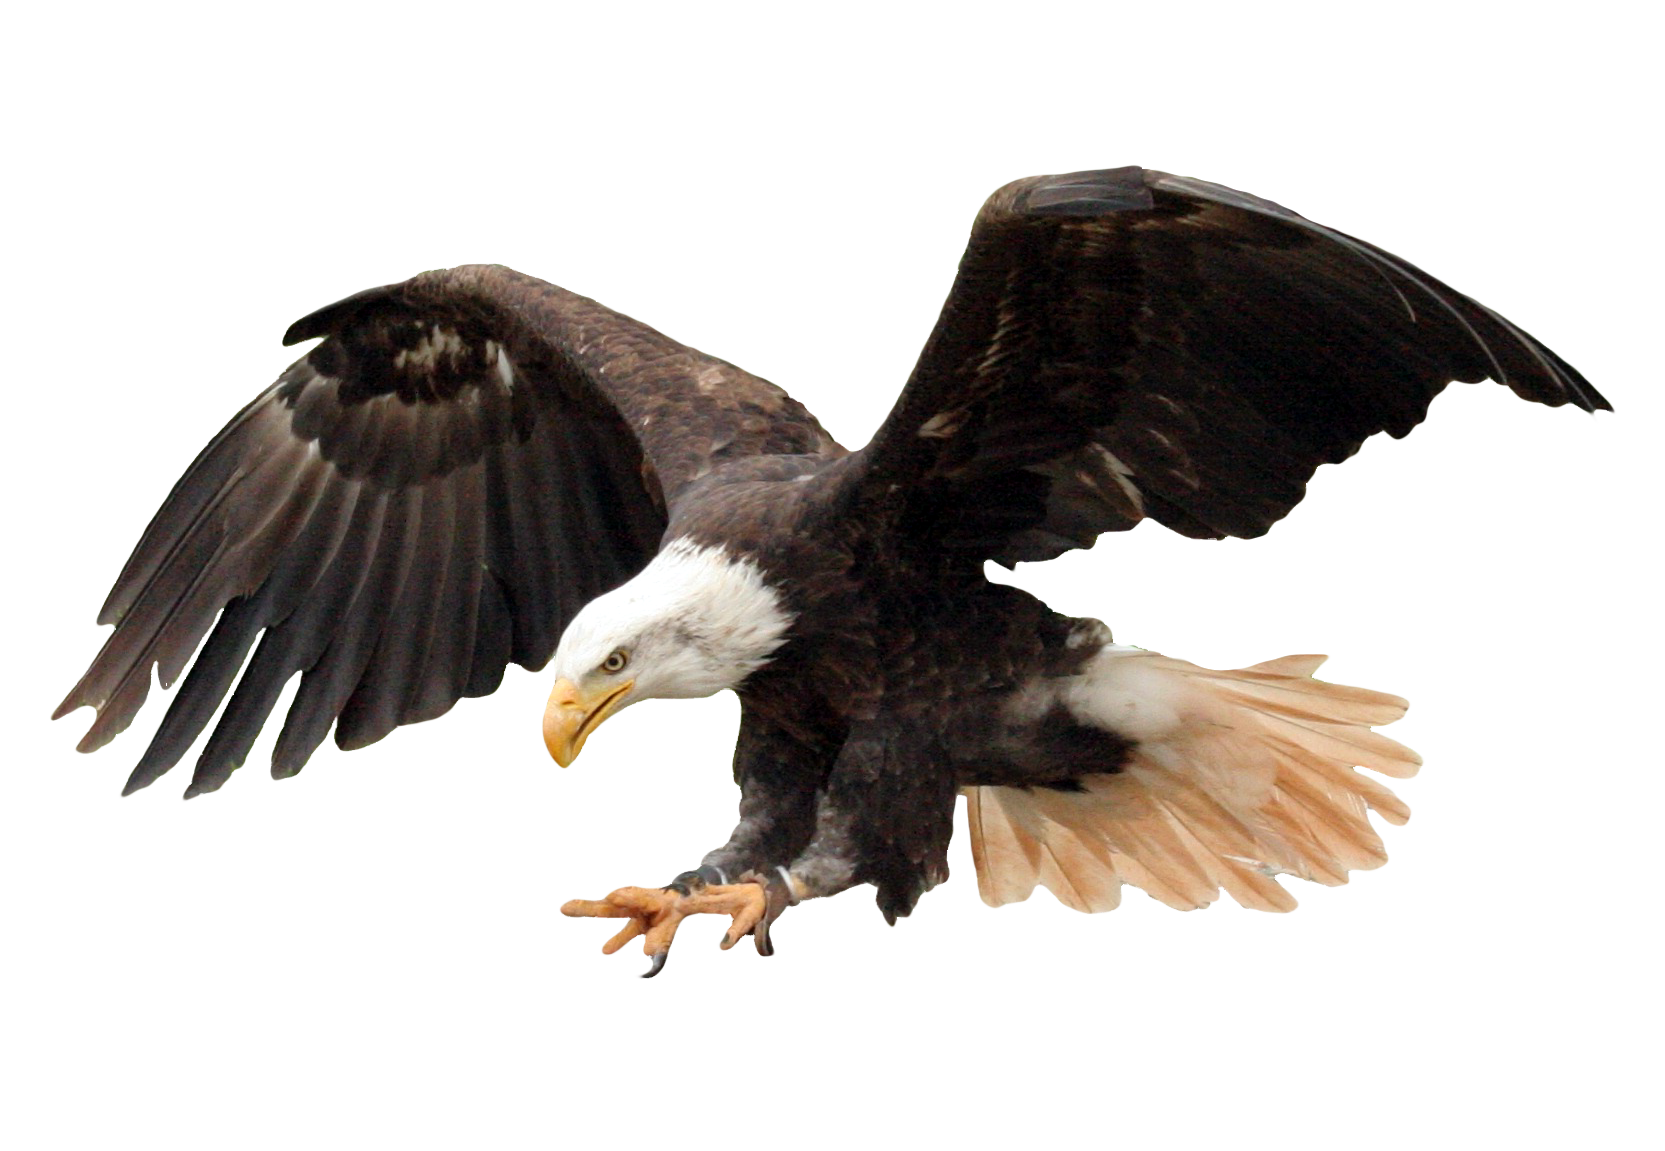
\includegraphics[width=200px,keepaspectratio]{./eagle.png}
  \caption{Imagen original}
  \label{fig:original}
\end{figure}

Una vez tenemos los datos de la imagen, obtenemos sus colores RGB y los guardamos en un dataframe. Además, damos valores a los ejes 'x' e 'y' a partir de las medidas de la imagen para representarlos de forma gráfica.

\begin{Schunk}
\begin{Sinput}
> coloresRGB <- data.frame(
+   x = rep(1:dims[2], each = dims[1]),
+   y = rep(dims[1]:1, dims[2]),
+   #as.vector:convierte matriz distribuida a vector no distribuido
+   R = as.vector(img[,,1]), 
+   G = as.vector(img[,,2]),
+   B = as.vector(img[,,3])
+   )
\end{Sinput}
\end{Schunk}

Por último, asignamos un cierto número de clústers para realizar la clasificación no supervisada, que en nuestro caso serán 2 (aunque puede ser cualquier número):

\begin{Schunk}
\begin{Sinput}
> numClust <- 2
\end{Sinput}
\end{Schunk}


\subsection{Algoritmo Kmeans}

Llamamos a la función kmeans() para realizar la clasificación según los colores obtenidos de la imagen. A continuación, creamos colores con rgb() a partir de los centroides obtenidos anteriormente:

\begin{Schunk}
\begin{Sinput}
> clasifKmeans <- kmeans(coloresRGB[, c("R", "G", "B")], centers = numClust)
> numColors <- rgb(clasifKmeans$centers[clasifKmeans$cluster,])
\end{Sinput}
\end{Schunk}

Una vez obtenidos los colores, los asignaremos a la gráfica que se creará con ggplot():

\begin{figure}[!htbp]
  \centering
  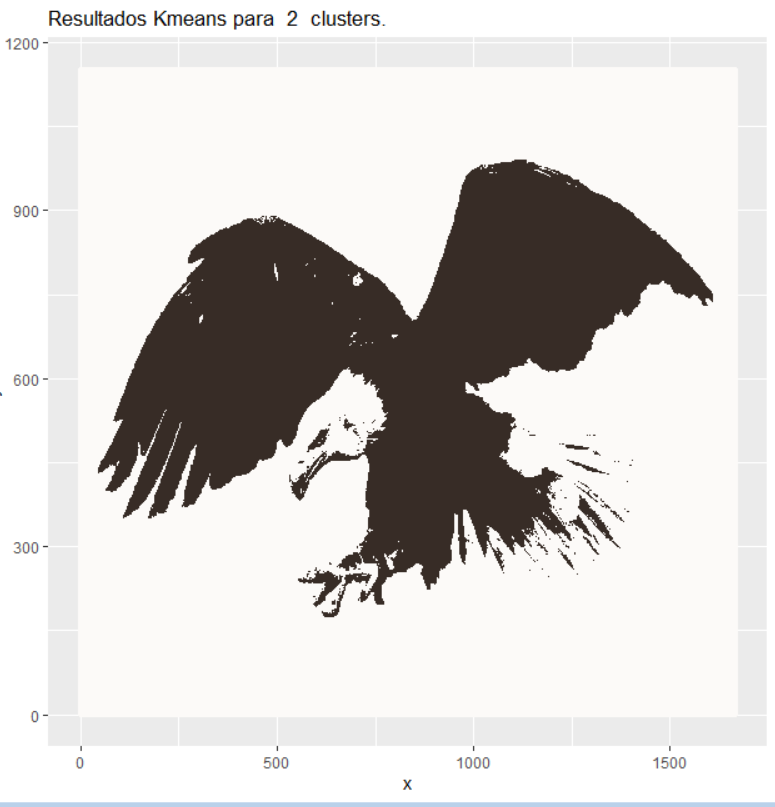
\includegraphics[width=200px,keepaspectratio]{./eagle2clusters.png}
  \caption{Imagen con 2 clusters}
  \label{fig:original}
\end{figure}


Si aumentamos el número de clústers y volvemos a realizar el algoritmo, la imagen toma más colores:

\begin{figure}[!htbp]
  \centering
  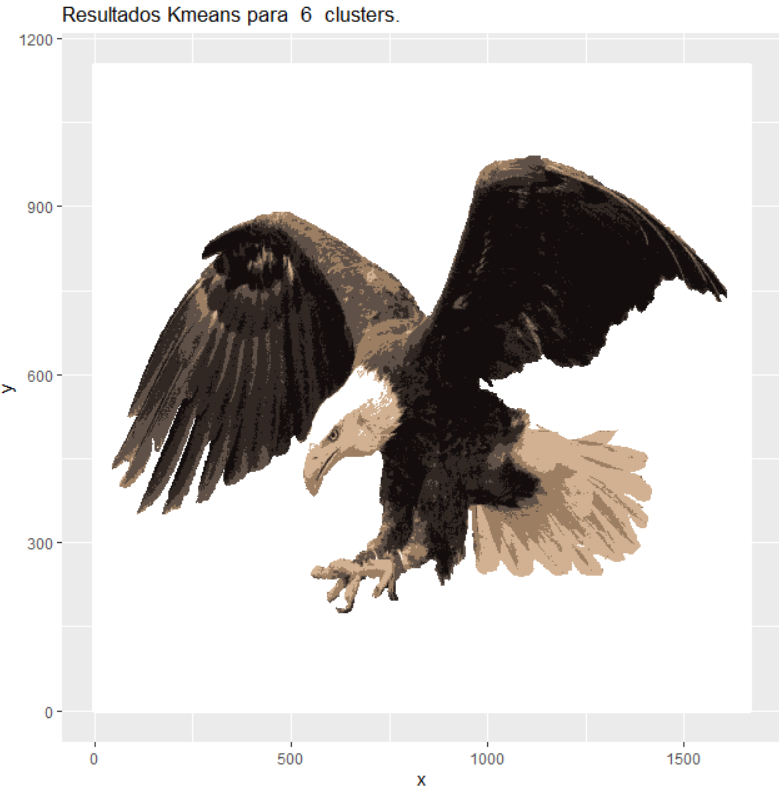
\includegraphics[width=200px,keepaspectratio]{./eagle6clusters.png}
  \caption{Imagen con 6 clusters}
  \label{fig:original}
\end{figure}

Cuantos más clústers se apliquen al algoritmo, más nitidez tendrá la imagen generada:

\begin{figure}[!htbp]
  \centering
  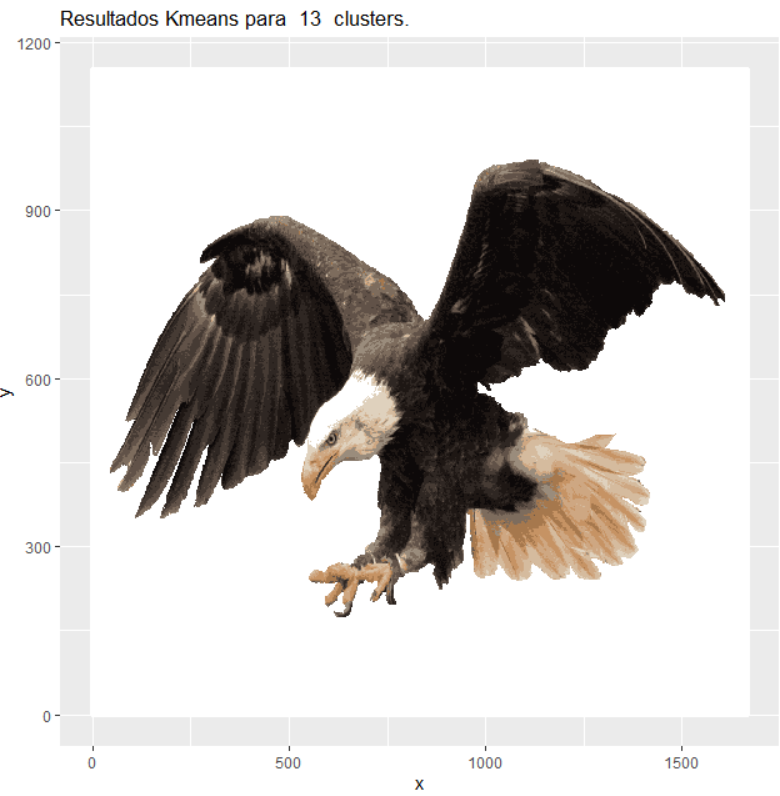
\includegraphics[width=200px,keepaspectratio]{./eagle13clusters.png}
  \caption{Imagen con 13 clusters}
  \label{fig:original}
\end{figure}

\newpage

\subsection{Algoritmo CLARA}

Para realizar el algoritmo CLARA, necesitamos instalar previamente las liberías cluster y factoextra:

\begin{Schunk}
\begin{Sinput}
> install.packages(c("cluster", "factoextra"))
\end{Sinput}
\begin{Soutput}
package ‘cluster’ successfully unpacked and MD5 sums checked
package ‘factoextra’ successfully unpacked and MD5 sums checked

The downloaded binary packages are in
	C:\Users\Javier\AppData\Local\Temp\RtmpAZ4Xc8\downloaded_packages
\end{Soutput}
\begin{Sinput}
> library(cluster)
> library(factoextra)
\end{Sinput}
\end{Schunk}

A continuación, llamamos a la función clara() para realizar la clasificación a partir de los colores del mismo dataframe utilizado para kmeans, que siga una métrica euclidean (también se pueden hacer cálculos con la métrica manhattan) y para un número de 10 muestras:

\begin{Schunk}
\begin{Sinput}
> clasifClara <- clara(coloresRGB, numClust, metric = "euclidean", stand = FALSE, samples = 10, pamLike = FALSE)
> clasifClara
\end{Sinput}
\begin{Soutput}
Call:	 clara(x = coloresRGB, k = numClust, metric = "euclidean", stand = FALSE,      samples = 10, pamLike = FALSE) 
Medoids:
        x   y         R         G         B
[1,]  472 596 0.2117647 0.1411765 0.1411765
[2,] 1331 569 1.0000000 1.0000000 1.0000000
Objective function:	 385.0042
Clustering vector: 	 int [1:1916415] 1 1 1 1 1 1 1 1 1 1 1 1 1 1 1 1 1 1 ...
Cluster sizes:	    	 1036817 879598 
Best sample:
 [1]   23862   45326   74627  130596  165014  198964  243149  245722  255840
[10]  402022  415707  506183  516213  542677  633708  634702  648533  672775
[19]  706024  710585  717984  795124  802961  844047  892881  995609 1045086
[28] 1155446 1276509 1310108 1313296 1319232 1430498 1493954 1495240 1531413
[37] 1535595 1567264 1577031 1737804 1776433 1814594 1825706 1832841

Available components:
 [1] "sample"     "medoids"    "i.med"      "clustering" "objective" 
 [6] "clusinfo"   "diss"       "call"       "silinfo"    "data"      
\end{Soutput}
\end{Schunk}


\newpage

Para visualizar los resultados obtenidos hacemos uso de la función fviz_cluster.

A la función, le asignaremos: los datos obtenidos de la clasificación con CLARA,
el tipo de elipse t, que asume una distribución de tipo t multivariable, el tipo de texto utilizado para representar los datos en la gráfica, 
que en nuestro caso será point de tal forma que solo se muestran los puntos en la gráfica sin etiquetas y la especificación del tamaño de los puntos representativos de los datos,
en el que se ha elegido un tamaño de 2.5 unidades.


\begin{figure}[!htbp]
  \centering
  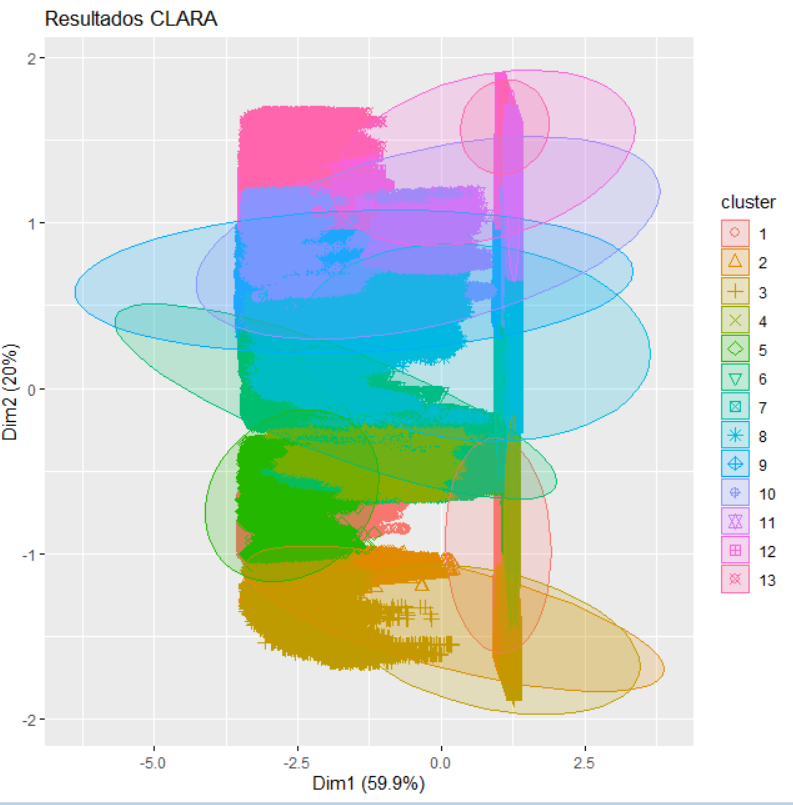
\includegraphics[width=250px,keepaspectratio]{./graficoClara.png}
  \caption{Imagen CLARA}
  \label{fig:original}
\end{figure}



\section{Tercera parte}

En esta última parte vamos a analizar y utilizar el paquete LearnClust, que contiene funciones que permiten hacer cálculos mediante algoritos de clustering jerárquico. Para ello, necesitamos instalar la librería LearnClust:

\begin{Schunk}
\begin{Sinput}
> install.packages("LearnClust")
\end{Sinput}
\begin{Soutput}
package ‘LearnClust’ successfully unpacked and MD5 sums checked

The downloaded binary packages are in
	C:\Users\Javier\AppData\Local\Temp\RtmpAZ4Xc8\downloaded_packages
\end{Soutput}
\begin{Sinput}
> library(LearnClust)
\end{Sinput}
\end{Schunk}

Para probar algunas funciones ofrecidas por esta libería, hacemos uso del enunciado del ejercicio realizado en la primera parte de esta práctica. Para el análisis de otras funciones se utilizarán otros ejemplos.

\subsection{AgglomerativeHC}

Esta función ejecuta el algoritmo de clustering jerárquico aglomerativo completo tomando como parámetros el tipo de distancia y aproximamiento en forma de string.

\begin{Schunk}
\begin{Sinput}
> m<-matrix(c(4,4, 3,5, 1,2, 5,5, 0,1, 2,2, 4,5, 2,1),2,8)
> agglomerativeHC(m,'EUC','MAX')
\end{Sinput}
\begin{Soutput}
$dendrogram
Number of objects: 2 


$clusters
$clusters[[1]]
  X1 X2
1  4  3

$clusters[[2]]
  X1 X2
1  4  5

$clusters[[3]]
  X1 X2
1  4  3
2  4  5


$groupedClusters
  cluster1 cluster2
1        1        2
\end{Soutput}
\end{Schunk}

\begin{Schunk}
\begin{Sinput}
> agglomerativeHC(m,'EUC','MAX')
\end{Sinput}
\begin{Soutput}
$dendrogram
Number of objects: 2 


$clusters
$clusters[[1]]
  X1 X2
1  4  3

$clusters[[2]]
  X1 X2
1  4  5

$clusters[[3]]
  X1 X2
1  4  3
2  4  5


$groupedClusters
  cluster1 cluster2
1        1        2
\end{Soutput}
\end{Schunk}
\includegraphics{Memoria-Figura 6: gráfica clustering aglomerativo}

\subsection{AgglomerativeHC.details}

Explica los pasos realizados en el algoritmo aglomerativo explicado en el apartado anterior sobre un conjunto de datos a resolver.

\begin{Schunk}
\begin{Sinput}
> agglomerativeHC.details(m,'EUC','MAX')
\end{Sinput}
\begin{Soutput}
[[1]]
     [,1] [,2] [,3]
[1,]    4    3    1

[[2]]
     [,1] [,2] [,3]
[1,]    4    5    1

     [,1] [,2]
[1,]    0    2
[2,]    2    0
  X1 X2
1  4  3
2  4  5
\end{Soutput}
\end{Schunk}

\subsection{toList}

Convierte un conjunto de datos numérico en una lista. Dicho conjunto de datos puede ser una matriz, un vector o un dataframe.

\begin{Schunk}
\begin{Sinput}
> lst<-toList(m)
> m
\end{Sinput}
\begin{Soutput}
     [,1] [,2] [,3] [,4] [,5] [,6] [,7] [,8]
[1,]    4    3    1    5    0    2    4    2
[2,]    4    5    2    5    1    2    5    1
\end{Soutput}
\end{Schunk}

\subsection{octileDistance}

Calcula la distancia octil entre dos clústers.

\begin{Schunk}
\begin{Sinput}
> x <- c(1,2)
> y <- c(1,3)
> octileDistance(x,y)
\end{Sinput}
\begin{Soutput}
[1] 1
\end{Soutput}
\end{Schunk}

\subsection{canberradistance}

Calcula la distancia de Canberra entre dos clústers.

\begin{Schunk}
\begin{Sinput}
> canberradistance(x,y)
\end{Sinput}
\begin{Soutput}
[1] 0.2
\end{Soutput}
\end{Schunk}

\section{Conclusiones}

El lenguaje R nos permite aplicar de forma sencilla y eficaz los algoritmos de clasificación no supervisada, además de que nos facilita representar de forma gráfica los resultados obtenidos de la aplicación de dichos algoritmos. En nuestro caso se han aplicado Kmeans y CLARA, en donde hemos podido comprobar que, aunque ambos algoritmos son de agrupamiento por particiones, CLARA es más apropiado para conjuntos muy grandes de datos mientras que Kmeans puede abarcar más tamaños. Por último, hemos probado el paquete LearnClust, que permite realizar cálculos a través de los algoritmos de agrupamiento jerárquico.










\end{document}
